\chapter{Future Work}
\label{ch:future_work}

Considering GRAPHINIUS an arbitrarily extendable computing platform (which uses graphs as underlying, universal data structures), there are many possibilities to build upon this work, ranging from small improvements to the introduction of fundamentally new infrastructure, transcending the use of contemporary graph libraries. 

The use of a centralized, Web based graphical workflow system will prove especially useful in exploiting and propagating the experience of individual users, as it bundles not only data, but also the settings and results of all experiments conducted on that platform.


\section{Parallel processing (CPU)}
\label{sect:parallel_cpu}

At the time of this writing (early 2016), real parallel processing inside the browser cannot be achieved without falling back to proprietary technologies like Google's \textit{native client} \citep{yee2009native}. Although it is true that the Web Worker specification has allowed for parallel execution of threads inside the browser for several years now, this model prohibits the use of a shared space of memory. This limitation renders any serious attempt at multiprocessing futile, as not does the main thread have to copy each argument over to a Web Worker, the Workers would also constantly have to communicate their progress back to the main thread. It is obvious that such an approach will simply result in unmanageable overhead.

A new model for SMMT (shared memory multi-threading) revolves around the emerging standard of WebAssembly (WASM), which can be compiled down to ASM and directly passed to the host kernel by the JavaScript Virtual Machine. Instead of writing WASM manually (which will be possible, too) the ideal approach is to rather code in a different language (C++, Typescript etc.) and compile the resulting code to WASM.


\section{Parallel processing (GPU)}
\label{sect:parallel_gpu}

An even faster - and already feasible - alternative is to conduct computations directly on the graphics hardware, which on modern computers (and even mobile devices) is capable of astonishing performance. The only hindrances to programming directly on the GPU via the web browser are 1) the mandatory usage of the GLSL (OpenGL Shader Language), 2) only complicated copying of data to and from the graphics card (no shared memory with the JSVM) as well as 3) the possible emergence of far superior ways of GPU coding (like WebCL), which would render extensive investments \& efforts today relatively useless in the near-future.


\section{General processing / ML pipelines}
\label{sect:pipelines}

As existing stacks indicate, there are several possible levels of pipelines which can be sorted by increasing homogeneity amongst their stages as well as decreasing technical demands on their users:

\begin{itemize}
	\item Level 0: Writing all of the pipeline manually. As every combination of technologies are usable, this approach gives the most flexibility but is hard to maintain and almost impossible to reproduce. As \citep{MLTechnicalDebt} perfectly states: ``Using self-contained solutions often results in a glue code system design pattern, in which a massive amount of supporting code is written to get data into and out of general-purpose packages.''
	
	\item Level 1: Automated, but self designed and coded. This entails the usage of tools like Unix Make, which is language agnostic and therefore supports any number of technologies as long as they are executable from a Shell. Apart from slightly better decoupling, same problems as Level 0.
	
	\item Level 2: Establishing a common understanding of the components and structure of a pipeline while still using individual technologies. Such a common standard exists in the form of PMML - the Predictive Model Markup Language. PMML defines stages of pipelines as well as their inputs, parameter types and ranges, the output format etc. Thus, developers can use their favorite technologies during development while PMML-consuming tools then produce familiar code (Hadoop, Spark etc.).
	
	\item Level 3: Language specific libraries exposing an API to conveniently assemble a pipeline. Such libraries have been released by projects like scikit-learn or Apache Spark. While currently becoming popular, APIs still restrict the creation of data applications to experts capable of coding.
	
	\item Level 4: The use of a custom DSL would widen the ability to create complex data pipelines to any kind of domain expert. Similar in nature to SQL, it is able to either compile itself into code or an intermediate representation like PMML.
	
	\item Level 5: A fully integrated data analysis platform that offers intuitive, visual pipeline assembly. Ideally, tools for reporting, reproduction and collaboration would also be included. In addition, the platform could offer experts the means to write stages themselves via an online code editor.
\end{itemize}

As many areas of applications for graph theory could make use of integrated processing pipelines 
\citep{MLPipelines}, the future of Graphinius could lie in providing a Level 5 experience.


\section{JSVM based grid computing}
\label{sect:jsvm_grid}

In order to process large graphs, single instances of the JSVM will no be sufficient. In order to make this scenario possible, it will be necessary to implement some form of internet-based cluster-approach, which is probably best defined by the term 'grid computing'. Unfortunately, most ML libraries are still not natively designed for distributed computing \citep{MLPipelineMLlib}.

A survey of economic models for grid brokers and schedulers was conducted in \citep{Abramson2002}. Although interesting in the long run, we will use a simple queue mechanism to demonstrate our platform.

\citep{Huang2006} argues that VM's for cloud computing have desirable properties including security, isolation and ease of configuration, but that the overhead of having to start/stop/migrate those instances impacts performance. Graphinius' virtual machines will be completely lightweight and can be managed by opening/closing a browser tab.

A list of top 10 obstacles for cloud computing can be found in \citep{Armbrust2010}. Although an exhaustive comparison to our approach is not possible at this point and matter of our research, most of these arguments stem from the fact that cloud data security as well as scalability are usually in the hands of powerful vendors.

\citep{Youseff2008} define an ontology of cloud computing encompassing five layers: hardware (fabric), software kernel (fabric management), cloud infrastructure (communication), cloud software environment (PaaS) as well as cloud application (SaaS, configuration without programming). This view is similar to our proposed pipeline levels before, where the implementation of Graphinius will start at about level 3.

\citep{Liu2012} and \citep{Liu2014} describe a distributed, scientific workflow system for bioinformatics based on a platform called Galaxy and its deployment to Amazons EC2 service via the Globus Provisioning framework; it supports graphical composition of workflows without requiring programming knowledge, which is especially interesting for less tech-savvy researchers. The concept of Galaxy is a very interesting one, although the author believes that client-side, GPU-enabled computations in coordination with one another are the future of personal and institutional grids.


\section{Heterogeneous data linkage}
\label{ssect:heterogeneous_data}

Many research fields comprise several sub-problems which are amenable to different machine learning approaches and feature their own, distinctive input data sets. Coming from various, different data sets featuring their distinct attribute domains, they probably are - via their time-, space- or other dimensions, interlinkable with one another. Usually, studies are only concerned about using a single one of those data sources and applying different methods to it. However, a more holistic approach would be to fuse those data sets along one or more dimensions (or any other meaningful ruleset) in order to achieve a richer representation of the underlying problem. A resulting data-set might take the form of a graph structure, in which individual entities from the originating sets are linked by meaningful connection rules, which in themselves will have to be learned.


\section{Meta machine learning}
\label{sect:meta_ml}

There are many papers in the Machine Learning community, Artificial Intelligence Planning, Operations Research and Hyper Heuristics (mostly for the optimization of search problems). From those papers it is clear that this field has a very rich history and therefore offers a plethora of research venues to be explored. As one of the first papers regarding this topic, \citep{Rice1975} defined the "Algorithm Selection Problem", which was first recognized as a meta learning problem by the machine learning community. He describes several spaces in which the Algorithm Selection Problem plays out:

\begin{itemize}
	\item \textbf{The problem space}: This is the set of all possible input problems (datasets + desired result class).
	
	\item \textbf{The feature space}: Features of a specific problem or family of problems. In dermatological imaging those would be defined by the imaging method (laser-scan vs. stanza), the scale of the objects to be detected (single cells vs nevi) etc.
	
	\item \textbf{The algorithm space}: The set of all algorithms suitable for the specific problem (features) to be worked on.
	
	\item \textbf{The performance measures} (the metric space): The set of possible measurements that could describe the quality of a solution (runtime performance, accuracy, ..).
	
	\item \textbf{The criteria space}: The weighing of different performance measures considered for a particular solution.
\end{itemize}

\cite{Horvitz2001} proposes a Bayesian learning algorithm that takes as input the generator function (assuming a generative model) of problem instances, the structure of input problems before solving, as well as the runtime behavior of a solver during execution in order to compute a Bayesian (posterior) score. The model was trained to predict runtime, but experiments showed that classification accuracy of the trained models could be significantly higher than that of the respective marginal model.

\cite{Hutter2007} note that manually sifting through parameter spaces of optimization algorithms is tedious work best suited for automated exploration. Interestingly, they see the selection of suitable building blocks in an algorithmic sequence (e.g. a preprocessing phase) as the same problem as setting parameters.

\cite{SmithMiles2008} proposes a meta-learning inspired framework for analyzing meta-heuristic algorithm performance by learning the correlation between fitness function evaluations (of a chosen lower-level algorithm) and search space characteristics. The sequence in this approach works as follows: Based on 1) definition of a problem and 2) its features, 3) different problem instances are instantiated (training data). 4) Applying different algorithms to those instances, 5) outcomes are measured by suitable performance metrics, thereby 6) gaining meta-knowledge about algorithmic performance. An experiment to learn those correlations by ANN showed that performance could be predicted rather accurately for different algorithms on instances of the Quadratic Assignment Problem.

In most scenarios concerning Graphinius we will be concerned with the selection of algorithmic components and their parameters based on the nature of the specific area of application, previously tackled problems, their features, available algorithms, preprocessing methods, parameters as well as performance measures.


\section{Hyper heuristics}
\label{sect:hyper_heuristics}

\cite{Burke:2003:Hyperheuristics} introduce hyper heuristics as being different from meta-heuristics in that they concern themselves with families / classes of problems rather than one specific problem domain. They search a heuristics space instead of a solution space and often the goal is finding general-purpose heuristics that do not need to be optimal, but rather good-enough, soon-enough, cheap-enough. They also describe the 'Domain barrier', a concept which refers to a hyper heuristics approach being oblivious of the underlying problem domain, but simply receiving a collection of low level heuristics and deciding which one(s) to use, based solely on past history of heuristics applied and objective function values returned.

From \citep{Burke2010}, we can take the idea of three 'dimensions' of the hyper heuristics recommendation problem:

\textbf{Selection vs. generation}, where selecting means applying existing heuristics to different (families of) problems, whereas generating new heuristics by assembling them from existing heuristic components (which first need to be decomposed from already known heuristics).

\textbf{Construction vs. perturbation}, where construction means starting with an algorithmic component and developing it iteratively by putting more and more components together. In contrast, perturbation means starting with a whole solution (or sequence of algorithms) and gradually transmuting it into a new solution.

\textbf{Online vs. offline learning}, where online means testing each new combination of algorithmic components on several problem instances to determine their fitness during the learning phase. This seems to be a good approach when immediate recommendation is not required and computing power is abundant. Offline learning, on the other hand, means selecting a ready-to-use (sequence of) heuristics and applying them to a set of training instances in the hope of gaining helpful insights from those experiments.

Although many research fields in themselves are not broad enough to be a suitable proving ground for hyper heuristic research, the Graphinius platform will provide us with meta-data about experiments in many diverse areas. We fully agree with \cite{Burke2013} who concludes that there is still little interaction between research communities, a problem whose solution could lead to the extension of algorithms to both new problem domains and new methodologies through cross-fertilization of ideas.


\section{Algorithmic recommender}
\label{sect:algo_recommender}

As a natural consequence of the previous sections, a recommender for graph theoretical Machine Learning pipelines would ideally take arbitrary problem instances and output a suitable processing pipeline which has worked well for similar problems in the past. In addition, the pipeline would also be directly configured in code and downloaded into a researcher's browser, making it available to immediate execution.


\section{Interactive Machine Learning}
\label{sect:fut_iml}

Last (but certainly not least), the problem of interactive machine learning lies in enabling a human domain-expert to exercise influence over the internal optimization considerations of a ML algorithm. For instance, if we take the SaNGreeA algorithm example of Section~\ref{sect:aoa_anonymization}, we can imagine multiplying the cost vector (representing the information loss of a data point's generalized quasi-identifiers) by an arbitrary weight vector, giving either one or the other data attribute precedence of being preserved. Following the approach in Figure~\ref{fig:anonIML}, we could use an appropriate UI to intervene it that process: everytime the algorithm has to make a clustering decision, it would instead (with a certain probability) present the domain expert with that choice - and learn the human's preferences by taking into account their answers, thereby manipulating the weights of the cost vector. It would be interesting to see how anonymization results would change, not only in appearance, but especially in their resilience against background-knowledge attacks as a result of such customizations.

\vspace{0.3cm}
\begin{figure}[ht]
	\begin{center}
		\hspace*{-2cm}
		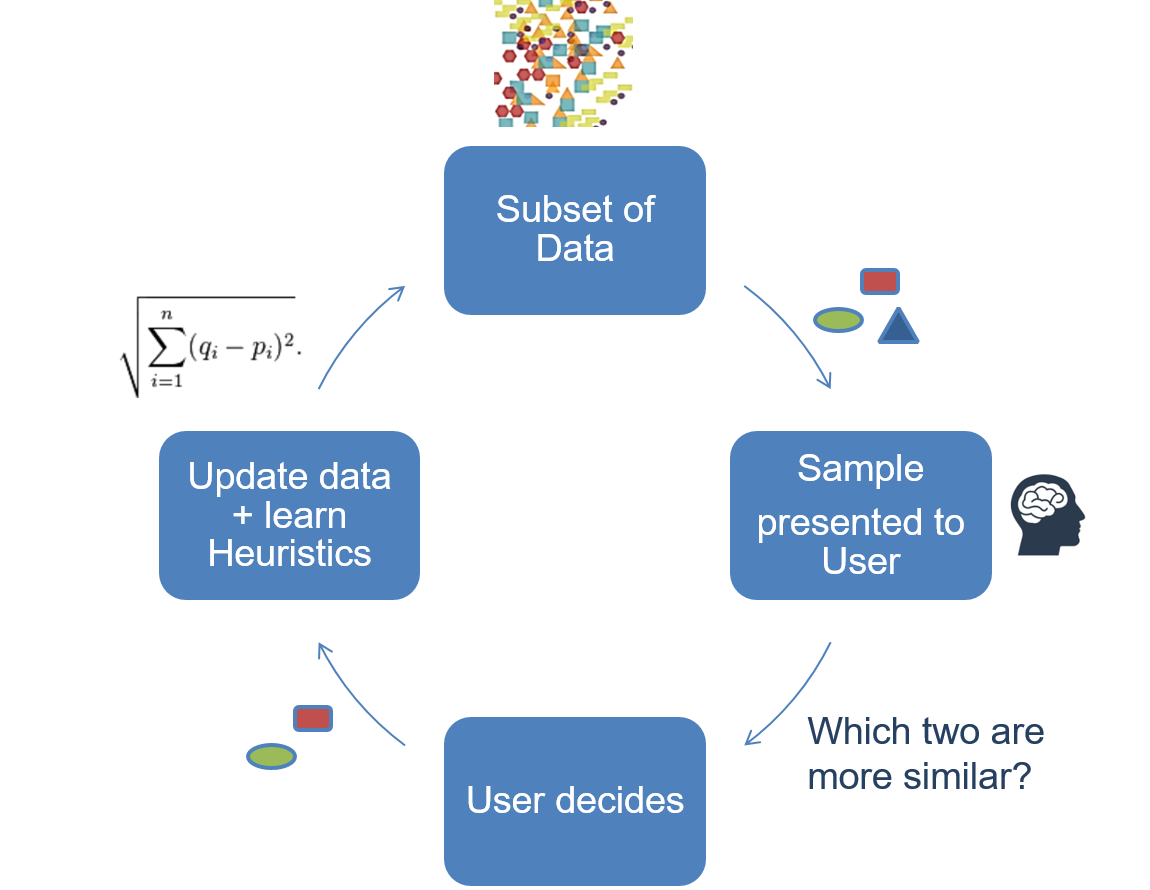
\includegraphics[width=1.2\textwidth]{figures/anonym/anonIML}
		\caption{Anonymization augmented by IML (human in the loop)}
		\label{fig:anonIML}
	\end{center}
\end{figure}
